\documentclass[12pt,letterpaper]{article}

\usepackage[margin=0.85in]{geometry}
\usepackage[T1]{fontenc}
\usepackage{lmodern}
\usepackage[scaled=0.95]{helvet}
\renewcommand{\familydefault}{\sfdefault}
\usepackage{amsmath}
\usepackage{array}
\usepackage{tabularx}
\usepackage{booktabs}
\usepackage[table]{xcolor}
\usepackage{enumitem}
\usepackage{tikz}
\usepackage[most]{tcolorbox}
\usepackage{titlesec}
\usepackage{fancyhdr}
\usepackage{needspace}

% ---------- Colors ----------
\definecolor{cookie}{HTML}{C68B4E}
\definecolor{cookiedark}{HTML}{7A4A22}
\definecolor{chip}{HTML}{3B2314}
\definecolor{monster}{HTML}{1F6FB5}
\definecolor{count}{HTML}{6B3FA0}
\definecolor{softyellow}{HTML}{FFF6DD}
\definecolor{softblue}{HTML}{E8F1FA}
\definecolor{softpurple}{HTML}{F1EBF8}
\definecolor{softgray}{HTML}{F3F3F3}

% ---------- Headings ----------
\titleformat{\section}{\Large\bfseries\color{cookiedark}}{}{0pt}{}
\titlespacing*{\section}{0pt}{14pt}{6pt}
\setcounter{secnumdepth}{0}

\pagestyle{fancy}
\fancyhf{}
\renewcommand{\headrulewidth}{0pt}
\fancyfoot[C]{\small\color{gray}The Cookie Countdown \textperiodcentered\ page \thepage}

\setlength{\parindent}{0pt}
\setlength{\parskip}{6pt}

% ---------- Helpers ----------
% A cookie with chocolate chips
\newcommand{\cookie}[1][1]{%
  \begin{tikzpicture}[scale=#1, baseline=-0.6ex]
    \fill[cookie] (0,0) circle (0.5);
    \draw[cookiedark, line width=0.8pt] (0,0) circle (0.5);
    \foreach \x/\y in {-0.2/0.2, 0.15/0.25, 0.25/-0.1, -0.1/-0.25, -0.28/-0.05, 0.05/0.0}
      \fill[chip] (\x,\y) circle (0.06);
  \end{tikzpicture}}

\newcommand{\blank}[1][3cm]{\underline{\hspace{#1}}}

\newcounter{question}
\newcommand{\question}{%
  \refstepcounter{question}\par\needspace{3\baselineskip}%
  \textbf{\color{monster}Question \arabic{question}.}~}

\newtcolorbox{bigidea}[1][]{enhanced, colback=softyellow, colframe=cookie,
  boxrule=1pt, arc=3mm, left=8pt, right=8pt, top=6pt, bottom=6pt,
  fonttitle=\bfseries, coltitle=white, colbacktitle=cookiedark, #1}
\newtcolorbox{tryit}{enhanced, colback=softblue, colframe=monster,
  boxrule=0.8pt, arc=3mm, left=8pt, right=8pt}
\newtcolorbox{calcclub}[1]{enhanced, colback=softpurple, colframe=count,
  boxrule=0.8pt, arc=3mm, left=8pt, right=8pt, top=4pt, bottom=4pt,
  title={\textbf{#1}}, colbacktitle=count, coltitle=white}

\renewcommand{\arraystretch}{1.6}

\begin{document}

% ================= Title =================
\begin{center}
  {\cookie[0.9]\hspace{0.6em}\cookie[0.9]\hspace{0.6em}\cookie[0.9]}\\[6pt]
  {\Huge\bfseries\color{cookiedark} The Cookie Countdown}\\[4pt]
  {\Large A Rates Worksheet}\\[6pt]
  {\small\color{gray} October 31, 2026 \textperiodcentered\ Nathaniel}
\end{center}

\vspace{2pt}
Name: \blank[6cm] \hfill Date: \blank[4cm]

% ================= The story =================
\section{The story}

The bakery just baked \textbf{15,000 chocolate chip cookies}. That is a LOT of cookies!

\textbf{\color{monster}Cookie Monster} sneaks in. He eats \textbf{20 cookies every minute}. Nom nom nom.

\textbf{\color{count}The Count} wants to count the cookies. But every time he looks up, there are
fewer! \emph{``Ah ah ah! The number keeps CHANGING!''}

Today we will help The Count. We will learn how to figure out how many cookies are left, even
while Cookie Monster is still eating.

% ================= Big idea =================
\section{Big idea: a rate is ``how much changes each minute''}

\begin{bigidea}
Cookie Monster eats at the same speed the whole time: 20 cookies, then 20 more, then 20 more.
That speed is called a \textbf{rate}.

The cookie pile goes \textbf{down} by 20 every minute. Mathematicians say the cookies are
\emph{changing} at a rate of \textbf{minus 20 cookies per minute}. The minus means
``getting smaller.''
\end{bigidea}

\begin{tryit}
\textbf{Try it!} Put 20 counters (beans, blocks, or paper cookies) in a pile. Take 20 away.
That was one minute of Cookie Monster!
\end{tryit}

\question Is the cookie pile getting bigger or smaller? \blank[4cm]

\vspace{4pt}
\question How many cookies does Cookie Monster eat in 1 minute? \blank[3cm]

% ================= Warm-up =================
\newpage
\section{Warm-up: a small plate of 100 cookies}

Before the giant bakery, let's practice with one plate of \textbf{100 cookies}. Cookie Monster
still eats 20 every minute. Help The Count fill in the table by counting \textbf{back} by 20s.

\begin{center}\renewcommand{\arraystretch}{1.9}
\rowcolors{2}{white}{softyellow}
\begin{tabular}{|>{\centering\arraybackslash}p{3.8cm}|>{\centering\arraybackslash}p{4.2cm}|>{\centering\arraybackslash}p{3.8cm}|}
\hline
\rowcolor{cookiedark}
\textbf{\color{white}Minutes gone by} & \textbf{\color{white}Cookies eaten so far} & \textbf{\color{white}Cookies left} \\
\hline
0 & 0  & 100 \\ \hline
1 & 20 & 80  \\ \hline
2 &    &     \\ \hline
3 &    &     \\ \hline
4 &    &     \\ \hline
5 &    &     \\ \hline
\end{tabular}
\end{center}

\question After how many minutes is the plate empty? \blank[2.5cm] minutes

\vspace{4pt}
\question Look at the ``Cookies left'' column. How much smaller does it get each row? \blank[1.7cm]

\begin{bigidea}
That number is the \textbf{rate}. It is the same in every row! That is the secret The Count needs.
\end{bigidea}

% ================= Related rates =================
\section{Related rates: the chocolate chips disappear too!}

Every cookie has \textbf{10 chocolate chips}. When a cookie disappears, its 10 chips disappear
with it. So the chips and the cookies are \emph{related}: if we know one rate, we can find the other.

\begin{center}
\begin{tabular}{c@{\hspace{1.2em}}c@{\hspace{1.2em}}c}
\cookie[0.8] & $\longrightarrow$ & 10 chips gone \\[4pt]
\cookie[0.8]\,\cookie[0.8] & $\longrightarrow$ & 20 chips gone \\[4pt]
\cookie[0.8]\,\cookie[0.8]\,\cookie[0.8] & $\longrightarrow$ & 30 chips gone \\
\end{tabular}

\textbf{Count by 10s!}
\end{center}

\question Cookie Monster eats 20 cookies in one minute. How many chips is that? Count by 10s
twenty times, or use 20 groups of 10. \blank[2.5cm] chips per minute

\vspace{4pt}
\question Which number goes down faster each minute: cookies or chips? \blank[3cm]

\begin{bigidea}
This is called \textbf{related rates}: two things change together, and one changes 10 times as
fast as the other.
\end{bigidea}

% ================= Big bakery =================
\newpage
\section{The big bakery: 15,000 cookies}

15,000 is too many to count one at a time, even for The Count! So we use groups. From the
warm-up, we know \textbf{one plate of 100 cookies lasts 5 minutes}.

\question 10 plates make 1,000 cookies. If each plate takes 5 minutes, how long do 10 plates
take? Count by 5s ten times.

\begin{center}
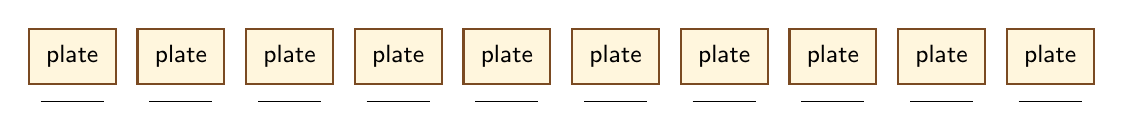
\begin{tikzpicture}[x=1.38cm]
  \foreach \i in {1,...,10} {
    \draw[cookiedark, line width=0.8pt, fill=softyellow] (\i-0.4,0) rectangle (\i+0.4,0.7);
    \node[font=\small] at (\i,0.35) {plate};
    \node[font=\small, below] at (\i,-0.05) {\blank[0.8cm]};
  }
\end{tikzpicture}
\end{center}

\hfill \blank[2.5cm] minutes

\question The bakery has 15 groups of 1,000 cookies. Each group takes the answer from
Question~7. Count by 50s fifteen times: 50, 100, 150, \ldots

\vspace{6pt}
\begin{center}
\renewcommand{\arraystretch}{1.9}
\begin{tabular}{|*{8}{>{\centering\arraybackslash}p{1.2cm}|}}
\hline
50 & 100 & 150 & & & & & \\ \hline
 & & & & & & & \cellcolor{softgray} \\ \hline
\end{tabular}
\end{center}

\hfill \blank[2.5cm] minutes

\question That is a long time! It is about 12 and a half hours. If Cookie Monster starts at
breakfast (7:00 in the morning), about when does he finish? Circle one:

\begin{center}

\begin{tikzpicture}
  \foreach \x/\lab in {0/Lunch time, 4.8/Dinner time, 9.6/Next week}
    \node[draw=cookiedark, rounded corners=6pt, line width=0.8pt, minimum width=3.6cm,
          minimum height=1cm, font=\large] at (\x,0) {\lab};
\end{tikzpicture}
\end{center}

\begin{tcolorbox}[enhanced, colback=white, colframe=cookie, boxrule=1pt, arc=3mm,
  height=6.5cm, title={\textbf{Draw it!}}, colbacktitle=cookie, coltitle=white]
Draw a big cookie pile. Draw an arrow pointing down and write ``$-20$ every minute'' next to it.
\end{tcolorbox}

% ================= Calculus Club =================
\newpage
\section{The Count's Calculus Club: write it like a scientist!}

\emph{``Ah ah ah! You just did CALCULUS!''} \textbf{Calculus} is the math of things that
\textbf{change}. Scientists use it for rockets, rivers, and the Sun. Here is how they write
what you already figured out.

\begin{calcclub}{Step 1: Give things short names}
Scientists use one letter as a nickname.
\begin{center}
\begin{tabular}{r@{\hspace{0.8em}}l}
$C$ & means the number of \textbf{C}ookies left \\
$t$ & means the \textbf{t}ime, in minutes \\
\end{tabular}
\end{center}
\end{calcclub}

\begin{calcclub}{Step 2: The ``change'' letter, $d$}
The letter $d$ means \textbf{``a little change in.''}
So $dC$ is a change in cookies, and $dt$ is a change in time. Put them together:
\[
  \frac{dC}{dt} = -20
\]
Say it out loud: \textbf{``dee-C dee-t equals minus twenty.''}
It means: \emph{the cookies change by $-20$ every minute.} That is the \textbf{rate} you found
in Question~4!
\end{calcclub}

\begin{calcclub}{Step 3: A rule for the cookies left}
For the plate of 100 cookies, the rule is
\[
  C = 100 - 20 \times t
\]
It says: start with 100, then take away 20 for every minute.
\end{calcclub}

\question Use the rule to find the cookies left after $t = 2$ minutes.
\quad $100 - 20 \times 2 = $ \blank[2cm]\\
Does it match your warm-up table? \blank[2.5cm]

\newpage
\begin{calcclub}{Step 4: Related rates, the scientist way}
Each cookie has 10 chips. If $P$ is the number of chi\textbf{P}s, then
\[
  \frac{dP}{dt} = 10 \times \frac{dC}{dt} = 10 \times (-20) = -200
\]
The chips go down 200 every minute: your answer to Question~5! Grown-up calculus students call
this the \textbf{chain rule}. You did it by counting by 10s.
\end{calcclub}

\begin{tcolorbox}[enhanced, colback=softblue, colframe=monster, boxrule=1pt, arc=3mm,
  title={\textbf{Super challenge!}}, colbacktitle=monster, coltitle=white]
Now The Count counts \textbf{60 cookies every minute} from the pile, and Cookie Monster
\emph{still} eats 20 every minute from the same pile.

\question How many cookies leave the pile each minute? \quad $60 + 20 = $ \blank[2cm]

When two things take from the same pile, their \textbf{rates add}! A scientist would write
\[
  \frac{dC}{dt} = -20 - 60 = -80
\]
With 15,000 cookies, the pile is empty after about 188 minutes:
that is about 3 hours instead of 12 and a half!
\end{tcolorbox}

{\small\color{gray}\textbf{For teachers:} the Step~3 rule is the solution of the differential
equation $dC/dt=-20$ with $C(0)=100$; for the bakery, $C(t)=15{,}000-20t$ reaches zero at
$t=750$ minutes (Question~8). In the challenge, $t = 15{,}000/80 = 187.5$ minutes, when The Count
has counted 11,250 cookies and Cookie Monster has eaten 3,750.}

% ================= Answer key =================
\newpage
\section{Answer key}

\begin{center}
\rowcolors{2}{white}{softyellow}
\begin{tabularx}{\linewidth}{|>{\centering\arraybackslash}p{2.8cm}|X|}
\hline
\rowcolor{cookiedark}
\textbf{\color{white}Question} & \textbf{\color{white}Answer} \\ \hline
1 & Smaller \\ \hline
2 & 20 cookies \\ \hline
Warm-up table &
  \begin{tabular}[t]{@{}lll@{}}
    Minute 2: & 40 eaten, & 60 left \\
    Minute 3: & 60 eaten, & 40 left \\
    Minute 4: & 80 eaten, & 20 left \\
    Minute 5: & 100 eaten, & 0 left
  \end{tabular} \\ \hline
3 & 5 minutes \\ \hline
4 & 20 smaller each row (the rate) \\ \hline
5 & 200 chips per minute \\ \hline
6 & Chips (10 times as fast) \\ \hline
7 & 50 minutes \\ \hline
8 & 750 minutes \\ \hline
9 & Dinner time (about 7:30 in the evening) \\ \hline
10 & 60 cookies; yes, it matches minute 2 of the table \\ \hline
11 & 80 cookies per minute \\ \hline
\end{tabularx}
\end{center}

\end{document}
